\section{Durchführung}
\label{sec:Durchführung}
Zur Bestimmung der Elementarladung $e$ mithilfe der Milikan-Metode wird ein Versuchsaufbau verwendet, der in \autoref{fig:aufbau} zu sehen ist. Die einzelnen Bauelemente werden in der Abbildung 
mit der jeweiligen Nummer bezeichnet. Wie in \autoref{sec:Theorie} beschrieben wird ein Plattenkondensator zur Erzeugung eines elektrostatischen Feldes benötigt. Dieses 
muss parallel zur Richtung der Gravitationskraft ausgerichtet sein. Der Experimentierraum ist mit Luft gefüllt. An der oberen Platte des Plattenkondensators befindet sich eine 
Öffnung, durch welche Öl in die Apparatur verstäubt werden kann. An der Seite des Plattenkondensators ist eine Halogenlampe installiert, um die Öltröpfchen besser sichtbar zu 
machen.
Unterhalb des Plattenkondensator befindet sich ein radioaktives $\alpha$-Präparat. Dieses kann über einen Hebel das Öl bestrahlen, um die Öltröpfchen zu ionisieren, sollte 
die Luftreibung nicht ausreichen, um eine Ladung der Tröpfchen zu erzeugen. Die Kammer des Plattenkondensators kann über ein anliegendes Mikroskop beobachtet werden. 
Durch welches die Öltröpfchen und ein Maßstab-Gitter zu sehen sind.
Der Abstand zweier \textit{dicker} Linien beträgt $\qty{0.5}{\milli\metre}$. Der Abstand zweier \textit{dünner} Linien zueinander beträgt 
$\qty{0.1}{\milli\metre}$.

\begin{figure}
    \centering
    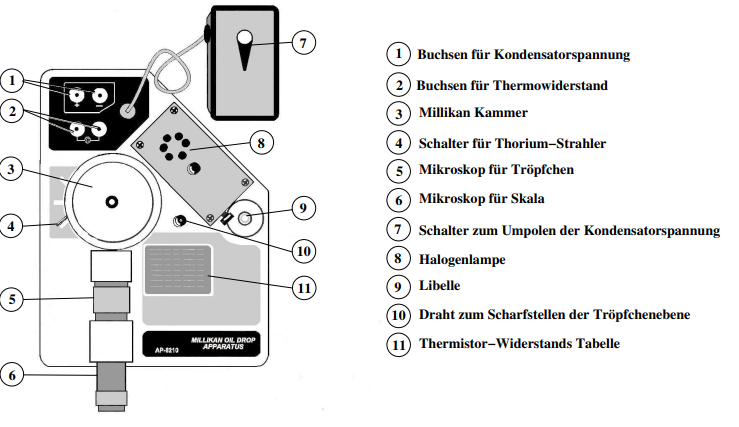
\includegraphics[width = \textwidth]{content/Aufbau.PNG}
    \caption{Skizze des Versuchaufbaus zur Untersuchung von Öltröpfchen im Magnetfeld. \cite{v503}}
    \label{fig:aufbau}
\end{figure}

Vor der Messung muss sichergestellt werden, dass die Messaparatur waagerecht ausgerichtet ist, um ungewünschte Abweichungen zu vermeiden. Es 
wird eine Spannung an den Kondensator angelegt, welche in einem Bereich von $\qty{100}{\volt}$ und $\qty{500}{\volt}$ liegen sollte. Bevor die Messung beginnt sollte die 
Lufttemperatur im Kondensator bestimmt werden, was über den Thermowiderstand vollzogen werden kann. Nun wird eine kleine Menge Öl in den Kondensator gesprizt. 
Dabei sollte das Feld abgeschaltet werden. Dies kann über den 
angeschlossenen Schalter geschehen, über welchen ebenfalls die Polung der Kondensatorplatten eingestellt werden kann. Wurde zu viel Öl in den Kondensator gesprizt ist die Beobachtung 
schwieriger. Daher sollte in diesem Fall das Öl abgelassen werden und nach fünf-minütiger Wartezeit erneut Öl eingeführt werden. 

Nun wird überprüft, ob sich geeignete Öltröpfchen im Kondensator befinden. Dafür wird die Bewegung der Öltröpfchen beobachtet. Bewegen diese sich in einer mäßigen 
Geschwindigkeit war die Injektion erfolgreich und die Messung kann beginnen. Sollte dies nicht der Fall sein, können die Öltröpfchen über den bereits erwähnten 
$\alpha$-Strahler ionisiert werden.

Das $\vec{E}$-Feld wird nun angeschaltet. Es wird die Zeit gemessen, in welcher sich der beobachtete Tropfen um eine bestimmt Strecke fortbewegt. Daraus kann eine Geschwindigkeit
berechnet werden. Anschließend wird das Feld umgepolt und es wird erneut eine Geschwindigkeit über dieselbe Methode gemessen. Die beiden Geschwindigkeiten entsprechen den 
Geschwindigkeiten $v_\text{auf}$ und $v_\text{ab}$, welche in \autoref{sec:Theorie} beschrieben wurden. 
Pro Tröpfchen werden beide Geschwindigkeiten jeweils drei mal gemessen. Des Weiteren wird die Gleichgewichtsgeschwindigkeit $v_0$ bei abgeschalteten 
$\vec{E}$-Feld bestimmt. Zu einer eingestellten Spannung des Kondensators wird diese Messung für fünf Tröpfchen durchgeführt. 
Es wird bei fünf verschiedenen Spannungen gemessen. Dabei ist zu beachten, dass die Temperatur während der Messung mehrmals notiert werden sollte, da diese sich im Verlauf
des Versuches ändern kann.
